\documentclass[12pt]{article}
\usepackage[czech]{babel}
\usepackage[utf8]{inputenc}
\usepackage[IL2]{fontenc}
\usepackage{wrapfig}
\usepackage{graphicx}
\usepackage{cprotect}


\begin{document}
%\setlength{\parindent}{0pt}
\begin{titlepage}

\includegraphics[scale=0.2, trim=5cm 0 0 30cm]{logo.jpg}
\begin{center}
\vspace{5cm}
{\Huge
\textbf{UIR}\\
\vspace{1cm}
}
{\Large
\textbf{KLASIFIKACE RUČNĚ PSANÝCH ČÍSLIC}
}
\end{center}
\vspace{\fill}

\begin{minipage}[t]{5cm}
\flushleft
Martin Hamet\\
Doba přípravy\texttt{ $\simeq$ 80h}
\end{minipage}
\hfill
\begin{minipage}[t]{7cm}
\flushright
\today
\end{minipage}
\end{titlepage}

\tableofcontents
\newpage
\section{Zadání}
\label{zadani}
Ve zvoleném programovacím jazyce navrhněte a implementujte program, který bude
schopen klasifikovat ručně psané číslice 0 - 9. Při řešení budou splněny následující podmínky:

\begin{itemize}
\item vytvoření trénovacích / testovacích dat pro učení / testování systému
\begin{itemize}
\item Každý student napíše alespoň jednu sadu cifer (pro tvorbu cifer použijte dodanou mřížku). Tyto budou dále oskenovány a převedeny do textového módu \texttt{.pgm} (rastr o velikosti 128 x 128 bodů nakreslených v 256 odstínech šedi). Vytvořená data budou uložena na sdílený disk, kde bude při ukládání dodržena následující konvence (osobní-číslo = adresář pro data každého studenta, v něm založit podadresáře 0 - 9, kde budou uloženy reprezentace jednotlivých cifer v uvedeném formátu). 
\end{itemize}

\item implementujte alespoň tři různé algoritmy (z přednášek i vlastní) pro tvorbu příznaků reprezentující číslice

\item implementujte alespoň dva různé klasifikační algoritmy (vlastní implementace, klasifikace bude s učitelem, např. klasifikátor s min. vzdáleností)

\item funkčnost programu bude následující:

\begin{itemize}
\item spuštění s parametry:
\\ \texttt{trénovací-množina testovací-množina 
\\parametrizační-algoritmus klasifikační-algoritmus 
\\název-modelu}\\
program natrénuje klasifikátor na dané trénovací množině, použije zadaný parametrizační a klasifikační algoritmus, zároveň vyhodnotí úspěšnost klasifikace a natrénovaný model uloží do souboru pro pozdější použití (např. s GUI).

\item spuštění s jedním parametrem \texttt{název-modelu} : program se spustí s jednoduchým GUI a uloženým klasifikačním modelem. Program umožní klasifikovat cifry napsané v GUI pomocí myši.
\end{itemize}

\item ohodnoťte kvalitu klasifikátoru na vytvořených datech, použijte metriku přesnost (accuracy). Otestujte všechny konfigurace klasifikátorů (tedy celkem 6 výsledků).

\end{itemize}


\section{Analýza problému a návrh řešení}
Úkolem je klasifikovat ručně psané číslice. Číslice mají být klasifikovány ze souborů ve formátu \texttt{.pgm} a prostřednictvím GUI tedy z nějaké bitmapy. Problém lze rozdělit na dvě hlavní části parametrizace a klasifikace. Parametrizace zajistí jednotný popis daného obrazu, který bude možné klasifikovat pomocí klasifikátoru. Protože chceme aby bylo možné zvolit si klasifikátor a parametrizační algoritmus nezávisle na sobě musíme sjednotit vstupní parametry klasifikátorů a výstupní popis parametrizací. Pro tento účel se nabízí jednorozměrný vektor o libovolné délce (příznakový vektor).

\subsection{Parametrizace}
Pro snazší zpracování bude vhodné reprezentace obrazů sjednotit do bitmapy (do které se obraz v případě formátu \texttt{.pgm} převede). Vzhledem k tomu že zpracováváme obraz ve 256 odstínech šedi je zbytečné používat klasickou bitmapu (s barevnými kanály A, R, G, B). Proto bude praktičtější vytvořit vlastní bitmapu i vzhledem k jednoduché práci s ní.

Formát \texttt{.pgm} (\texttt{PGM P2}) je v podstatě textově zapsaná podoba bitmapy, kde jsou na prvních čtyřech řádcích uloženy informace o obrazu (rozměry a maximální hodnota určující obvykle bílou barvu). Dále následují hodnoty určující barvy v jednotlivých pixelech. Jediný problém který z tohoto formátu plyne je že není příliš striktní. Čtení takto uloženého obrazu musí být s nadsázkou volnější. Některé obrazové editory ukládají jednu hodnotu na řádek jiné různě řádky zalamují apod.

Při vytváření bitmapy není úplně zřejmé zda je lepší ponechávat hodnotu pixelu takovou jaká je (tj. hodnota 0 - 255), nebo diskretizovat a pomocí nějaké meze určit zda bude hodnota 0 nebo 255 (vytvořit tedy čistě černobílý obraz bez odstínů).
Pomocí dobře zvolené meze pro určení zda má být pixel černý nebo bílý se dají z obrazu odstranit nechtěné ruchy okolí (okraje podél obrazu šum v případě nekvalitního skenování atp.), ale také by se mohli ztratit důležité části vlastní napsané číslice pokud by byla napsaná například světlou tužkou. Obecně by mohlo být vhodné použít kombinaci obou přístupů.

Dále pro minimalizaci nezajímavých částí obrazu (tj. bílých okrajů kolem číslice atp.) použijeme tzv. "MinMax obdelník". Tento obdélník vytvoříme tak, že si uložíme maximální/minimální index  pixelu který považujeme za černý) pro sloupce i řádky. 

\pagebreak

Pomocí těchto indexů vymezíme efektivní plochu obemykající číslici v obrazu, kterou budeme dále zpracovávat (viz obr.\ref{obr1} zelený obdelník).

Parametrizace tedy určí parametrizační vektor podle zvolené metody (viz dále) z bitmapy, kterou vytvoříme načtením ze souboru nebo triviálním převodem z bitmapy vytvořené kreslením v GUI.

\subsubsection{Řádkové průměrování (\texttt{WEIGHT)}}
\begin{wrapfigure}[12]{r}{5cm}
\centering
\vspace{-0.5cm}
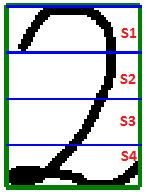
\includegraphics[height=4cm]{WeightSections.png}
\caption{Rozdělení obrazu na sekce.}
\label{obr1}
\end{wrapfigure}
Tento způsob je velmi jednoduchý a zjistí průměrnou hodnotu intenzity v každém řádku bitmapy. V našem případě by tedy vzniklo 128 hodnot což by bylo příliš jemný popis obrazu a nemusel by dobře popisovat číslice obecně (malé rozdíly by působily velké odlišnosti). Budeme tedy dále průměrovat řádky mezi sebou tak že rozdělíme bitmapu na požadovaný počet sekcí (viz obr.\ref{obr1} sekce \texttt{S1 - S4}) a v každé sekci zprůměrujeme všechny příslušné řádky. Tímto způsobem dostaneme číslo pro každou sekci, které udává poměr bílé a černé barvy v dané sekci. V tomto případě je obrázek rozdělen na čtyři sekce příznakový vektor tedy bude obsahovat číslo pro každou. Tím jsme značně zkrátili příznakový vektor a jak je vidět na obr.\ref{obr1} tento popis by měl sloužit dobře k rozlišení mezi čísly která se ve vertikálním směru značně liší v počtu černých pixelů na sekci (např. čísla 9 a 6).

Protože se jedná o horizontální průměrování nezáleží na horizontálním posunu nebo šířce číslice. Rozdělení na velké sekce může působit problémy např. v případě číslice 4 záleží zda vodorovná čára padne do sekce \texttt{S3} nebo \texttt{S4}.
\pagebreak

\subsubsection{Vzorkování (\texttt{SAMPLE})}
\begin{wrapfigure}[11]{r}{5cm}
\centering
\vspace{-0.5cm}
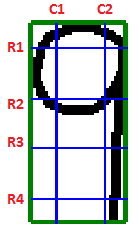
\includegraphics[height=4cm]{Samples.png}
\caption{Vzorky obrazu.}
\label{obr2}
\end{wrapfigure}

Jedná se podobný přístup jako v řádkovém průměrování s tím rozdílem že tentokrát nebudeme průměrovat řádky mezi sebou, ale vezmeme pouze reprezentativní vzorky řádek. Zvolíme vzorky řádek a sloupců a zjistíme tedy poměr bílé a černé barvy ve vybraných řádcích/sloupcích. Vzorky vybíráme rovnoměrně a pouze z efektivního obdélníku (zelený obdélník) (viz obr.\ref{obr2}). Na obrázku jsou znázorněny vzorky řádek \texttt{R1 - R4} a vzorky sloupců \texttt{C1 a C2}. Průměry z jednotlivých řádek a sloupců zařadíme postupně do parametrizačního vektoru. Výsledný parametrizační vektor \texttt{P} by v tomto případě vypadal \texttt{P = [AR1, AR2, AR3, AR4, AC1, AC2]}, kde \texttt{A} značí aritmetrický průměr hodnot (intenzity) na příslušném řádku/sloupci.

Tento přístup umožňuje lepší rozlišení v horizontálním směru oproti metodě řádkového průměrování. V podstatě z výsledného vektoru můžeme určit kolikrát číslice prošla daný vzorkem pokud by jsme znali tloušťku čáry kterou je číslice napsaná. Protože se ale tato tloušťka projeví v každém vzorku jedná se o vynásobení výsledného vektoru konstantou čímž vznikne rovnoběžný vektor. Bylo by možné pokusit se o předzpracování obrazu tak aby tloušťka číslice byla pouze jeden pixel, potom by jsme skutečně dostali počet průniků se vzorkem. Pro zachování jednoduchosti zůstaneme u původního řešení.

Podobně jako u předchozí metody při zvolení velkého počtu vzorků bude metoda špatně zobecňovat číslice a při malém počtu by měli různé číslice příliš podobný výsledný parametrizační vektor.
\pagebreak

\subsubsection{Histogram orientovaných gradientů (\texttt{HOG})}
Tato metoda je založená na principu orientace gradientů v různých částech obrazu. Nejprve je nutné si uvědomit že pomocí gradientu v obrazu můžeme zjistit směr a sílu změny (intenzity barvy) v nějakém směru.

\begin{wrapfigure}[12]{l}{5cm}
%\vspace{-0.5cm}
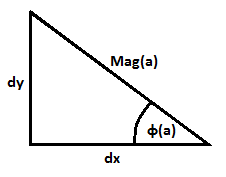
\includegraphics[width=5cm]{Gradient.png}
\caption{Gradient v bodě.}
\label{obr3}
\end{wrapfigure}

Aby jsme mohli určit gradient v některém bodě musíme nejprve určit hodnotu změny (derivaci) v horizontálním směru. To znamená zjistit změnu hodnoty \texttt{h} (v našem případě intenzita) předchozího a následujícího pixelu. Řekneme-li že chceme hodnotu derivace \texttt{dx} v pixelu \texttt{a} se souřadnicemi \texttt{[x, y]} použijeme vztah $dx(a) = h([x+1, y]) - h([x-1, y])$ stejně jako kdyby jsme detekovali hrany. Takto by jsme mohli pouze určit směr doleva nebo doprava. Pokud chceme určit směr ve rovině je nutné spočítat i derivaci ve vertikálním směru $dy(a) = h([x, y+1]) - h([x, y-1])$. Nyní můžeme určit gradient. Jak je znározněno na obrázku obr.\ref{obr3} pomocí pravidel v pravoúhlém trojúhelníku spočítáme směr největší změny 
{$\phi(a) = \tan^{-1}(\frac{dy(a)}{dx(a)})$} a její sílu v tomto směru $Mag(a) = \sqrt{dx(a)^2 + dy(a)^2}$.

\begin{wrapfigure}[13]{r}{5cm}
\vspace{-0.5cm}
\centering
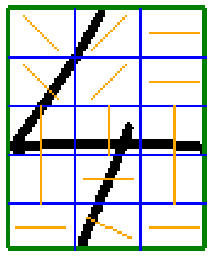
\includegraphics[width=4cm]{Hog.png}
\caption{\texttt{HOG} gradienty v sekcích}
\label{obr4}
\end{wrapfigure}

Když se zamyslíme nad směrem největší změny v našem případě není žádoucí určovat směr ve všech směrech roviny. V případě tenké rovné čáry by se od sebe gradienty odečetli protože by měli vzájemně opačný směr, proto budeme brát směr v absolutní hodnotě. Zajímá nás tedy směr největší změny ve \texttt{180$^{\circ}$}. Aby jsme mohli tvořit histogram těchto úhlů musíme je diskretizovat (např. po 30$^{\circ}$ dostaneme 6 částí). Každý pixel přispěje podle svého gradientu svou silou do příslušného úhlu (nejlépe váženým podílem do dvou nejbližších úhlů). 

Nyní už by jsme mohli vytvořit takový histogram pro celý obraz. Tím bychom ale přišli o informaci pozice jednotlivých gradientů. Aby jsme tuto informaci částečně zachovali rozdělíme efektivní oblast obrazu ještě do sekcí a pro každou sekci vytvoříme vlastní histogram (viz obr.\ref{obr4}).

\subsection{Klasifikace}
Při parametrizaci jsme získali vektor pro každý obraz, který ho podle zvolené parametrizační metody popisuje. V klasifikační části potřebujeme určit do jaké klasifikační třídy zařadit vektor na základě trénovacích dat, kde známe správný výsledek. Je tedy třeba klasifikátor připravit (vytvořit model) v trénovací části tak, aby s co největší přesností určil správnou třídu bez znalosti výsledku. Klasifikátor musí být také schopen takto vytvořený model uložit a případně později načíst, proto budeme volit jednoduché datové struktury. Pro účely ukládání bude vhodnější formát \texttt{XML} místo \texttt{TXT} vzhledem k přehlednosti uložených dat.

\subsubsection{Etalonový klasifikátor (\texttt{DISTANCE})}
Tento klasifikátor nejprve načte všechna trénovací data a poté je zpracuje a vytvoří vzorový parametrizační vektoru pro každou klasifikační třídu. Při testovací fázi už pouze počítá vzdálenost vzorů (etalonů) od testovaného vektoru (ze zkoumaného obrazu). Podle etalonu s nejkratší vzdáleností od testovaného zařadí testovaný vektor do příslušné třídy. Jedná se o jednoduchý klasifikátor, kde ovšem záleží na správném vytvoření etalonů.

Nejjednodušší způsob určení etalonů je průměr v dané klasifikační třídě z vektorů vytvořených z trénovacích dat. Výhodou je že po trénovací fázi není nutné uchovávat všechna trénovací data, ale pouze výše zmíněné etalony a je tedy tento klasifikátor paměťově významně úsporný.

Pro vypočítání vzdálenosti v našem případě příznakových vektorů můžeme použít Euklidovskou vzdálenost. Je tedy důležité aby se po celou dobu funkce tohoto klasifikátoru používal stejný parametrizační algoritmus, který produkuje vektory o stejné délce.

\subsubsection{K nejbližších sousedů (\texttt{KNN})}
Tento klasifikátor nevyžaduje žádné předzpracování trénovacích vektorů a pouze je zařazuje do své datové struktury podle jejich příslušnosti ke správné třídě. Testování dále probíhá na principu zjištění vzdálenosti (také Euklidovská vzdálenost) ke každému z trénovacích případů. A podle četností tříd v \texttt{K} nejbližších případech rozhodne do které třídy zkoumaný vektor zařadí.

Tento klasifikátor vyžaduje větší množství trénovacích dat, ale dokáže zpracovat různorodější třídy v našem případě různě psané číslice lépe. Tato výhoda sebou ovšem nese nevýhodu paměťové náročnosti protože je nutné, aby klasifikátor měl přístup ke všem trénovacím vektorům po celou dobu provozu. U takového klasifikátoru by mohla hrát významnou roli délka příznakového vektoru (matice, apod.). Tento klasifikátor je také kvůli množství dat pomalejší než např. Ethalonový klasifikátor.

\section{Implementace (popis řešení)}
Program je sestaven tak, aby bylo snadné ho rozšířit o další klasifikátory a parametrizační algoritmy a zajištění snadného upravení již existujících (viz dále).

\subsubsection{Hlavní moduly programu} 

\paragraph{\texttt{Form1}}
zajišťuje funkčnost GUI a poskytuje nástroje pro volání vykreslení atp.

\paragraph{\texttt{Program}}
zajišťuje hlavní funkci programu spuštění podle zadaných parametrů načítání, testování dat a spuštění GUI. Vytvoří novou instanci klasifikátoru a deskriptoru (parametrizační algoritmus). Posílá načtená data do klasifikátoru pro natrénování a následně pro testování. Obsahuje pouze jednu veřejnou metodu \texttt{evaluateBitmap()}, která je volaná prostřednictvím GUI pro vyhodnocení ručně napsané číslice v GUI reprezentované bitmapu.

\paragraph{\texttt{BWImage}}
obaluje vlastní bitmapu obrazu. Umožňuje vytvoření instance podle cesty k souboru (obrázku ve formátu \texttt{PGM P2}) nebo podle bitmapy. Při načítání jsou ukládány hodnoty o minimálních a maximálních indexech pro pozdější vytvoření MinMax obdélníku. Poskytuje možnosti převodu bitmapy do bitmapy kompatibilní s GUI pro vykreslení a získání výše zmíněných indexů.

\paragraph{\texttt{IDescriptor}}
poskytuje rozhraní pro jednotné ovládání deskriptorů.
\begin{itemize}
\item \texttt{getDescription()} vytvoří parametrizační vektor z předaného obrazu pomocí \texttt{BWImage}.
\item \texttt{getDescriptionVectorLength()} vrátí délku parametrizačních vektorů které vytváří
\end{itemize} 

\paragraph{\texttt{ICLassifier}}
poskytuje rozhraní pro jendotné ovládání klasifikátorů.
\begin{itemize}
\item \texttt{addTrainCase() přidá do klasifikátoru nový vektor se správnou třídou}. Pomocí této metody se trénuje klasifikátor.
\item \texttt{evaluate()} vytvoří vektor (descriptorem klasifikátoru) z předaného obrazu \texttt{BWImage} a klasifikuje ho. Metoda vrací číslo třídy do které byl tento vektor klasifikován.
\item \texttt{saveModel()} uloží natrénovaný model do souboru ve formátu \texttt{XML} pro pozdější použití.
\item \texttt{loadModel()} načte natrénovaný model ze souboru a připraví tak klasifikátor na vyhodnocování.
\end{itemize}

\paragraph{\texttt{WeightDescriptor}}
reprezentuje parametrizační algoritmus řádkového průměrování. Pomocí konstanty \texttt{DESCRIPTION\_LENGTH} lze nastavit délka výsledného vektoru a tím i počet sekcí na které se obraz rozdělí. Descriptor nejprve vytváří vektor o délce 128 (původní výška obrazu) a dále ho normalizuje na danou hodnotu metodou \texttt{getNormalizedDescription()}.

\paragraph{\texttt{SampleDescriptor}}
reprezentuje parametrizační algoritmus vzorkování. Pomocí konstant \texttt{EXAMINED\_ROWS} a \texttt{EXAMINED\_COLUMNS} lze nastavit počet vzorků na řádek a sloupec. Délka výsledného vektoru je udaná součtem těchto konstant. Deskriptor nejprve zjistí indexy řádků a sloupců v efektivním obdélníku podle počtu požadovaných vzorků metodou \texttt{getSamples()}. Dále projde tyto řádky a sloupce v předaném obrazu \texttt{BWImage} a vytvoří výsledný vektor.

\paragraph{\texttt{HOGDescriptor}}
reprezentuje parametrizační algoritmus histogramu orientovaných gradientů. Pomocí konstant \texttt{BUCKET\_ROWS} a \texttt{BUCKET\_COLUMNS} lze nastavit počet sekcí na které se obraz rozdělí a tím počet histogramů na celý obraz což ovlivňuje délku výsledného vektoru. Konstantou \texttt{HISTOGRAM\_ANGLES} lze ovlivnit jemnost diskretizace směru gradientu. Descriptor prochází obraz \texttt{BWImage} a pro každý pixel zjistí jeho gradient a sekci do které patří metodou \texttt{getIndexOfBucket()} a přispěje váženou hodnotou gradientu do příslušné sekce a jejího histogramu. Výsledný vektor je potom vytvořen serializací histogramů ze všech sekcí.

\paragraph{\texttt{\texttt{DistanceClassifier}}}
reprezentuje etalonový klasifikátor. Přidávané trénovací vektory ukládá do seznamů ve slovníkové struktuře tak, že klíčem je správná klasifikační třída. Při prvním zavolání metody \texttt{evaluate()} se projdou všechny trénovací vektory metodou \texttt{compileReadings()} a vytvoří se příslušné etalony do seznamu \texttt{finalPatterns}. Při ukládání modelu zanikají informace o trénovacích vektorech a ukládá se pouze seznam etalonů.

\paragraph{\texttt{NearestNeighborClassifier}}
reprezentuje klasifikátor K nejbližších sousedů.
Přidávané trénovací vektory ukládá do seznamů ve slovníkové struktuře, tak že klíčem k seznamu je správná klasifikační třída. Stejně jako předchozí klasifikátor ovšem při ukládání se žádná informace neztrácí a veškeré trénovací případy se zachovávají.

\section{Uživatelská příručka}

\subsubsection{Formát uložených dat}
Formát obrazů ve formátu \texttt{PGM P2} viz \ref{zadani} Zadání.

\paragraph{Trénovací a testovací data}
musejí být uložena tak, že složka obsahuje podsložky 0 - 9 a v každé podsložce jsou samotné obrazy. Každý obraz musí být umístěn v takové složce která odpovídá jeho správné klasifikační třídě, aby bylo jasné co za třídu klasifikátor právě trénuje. Stejně u testovacích dat kde je toto umístění nutné pro určení přesnosti klasifikace. Na vlastních názvech souborů nezáleží je pouze nutná koncovka \texttt{.pgm}.

\pagebreak

\subsection{Spuštění programu}
Program se spouští z příkazové řádky. Jsou dvě možnosti spuštění. Program je napsaný v jazyce \texttt{C\#} bude tedy nutné pros spuštění mít stažené knihovny \texttt{Mcrosoft .NET Framework}.

\begin{itemize}
\item \texttt{NumberClasification.exe arg1 arg2 arg3 arg4 arg5}
\begin{itemize}
\item \texttt{arg1} název složky s trénovacími daty
\item \texttt{arg2} název složky s testovacími daty
\item \texttt{arg3} zkratka vybraného parametrizačního algoritmu (viz \ref{Descriptors})
\item \texttt{arg4} zkratka vybraného klasifikátoru (viz \ref{Classifiers})
\item \texttt{arg5} název souboru do kterého se natrénovaný model uloží
\end{itemize}

\item \texttt{NumberClasification.exe arg1}
\begin{itemize}
\item \texttt{arg1} název souboru s modelem který se má načíst
\end{itemize}

\end{itemize}

Příklad spuštění by mohl například vypadat takto:\\
\texttt{NumberClasification.exe TrainingData TestingData HOG DISTANCE ulozenyModul}

Po spuštění programu prvním způsobem se načtou trénovací data proběhne natrénování klasifikátoru podle zvolených parametrů. Dále se načtou testovací data proběhne testování a je do konzole vypsán výpis o úspěšnosti. Natrénovaný model se poté uloží do aktuální složky se jménem zadaným v parametrech.

Pro spuštění programu druhým způsobem je třeba mít již uložený natrénovaný model. Program načte model připraví se klasifikační a parametrizační algoritmy které byli použity při ukládání modelu a zobrazí jednoduché uživatelské rozhraní (viz \ref{GUI}).

Při spuštění programu s chybným počtem parametrů se zobrazí nápověda.

\pagebreak

\subsubsection{Zkratky parametrizačních algoritmů}
\label{Descriptors}
\begin{itemize}
\item \texttt{WEIGHT} řádkové průměrování
\item \texttt{SAMPLE} vzorkování
\item \texttt{HOG} histogram orientovaných gradientů
\end{itemize}

\subsubsection{Zkratky klasifikačních algoritmů}
\label{Classifiers}
\begin{itemize}
\item \texttt{DISTANCE} etalonový klasifikátor
\item \texttt{KNN} klasifikátor K nejbližších sousedů
\end{itemize}

\subsubsection{Grafické uživatelské rozhraní GUI}
\label{GUI}
Po spuštění GUI je okamžitě možné sním pracovat.
Do bílého panelu uprostřed je možné levým tlačítkem kreslit (resp. psát) pravé tlačítko myši umožňuje gumování. Plátno je interaktivní ve smyslu změny velikosti okna. Při nepoměrné velikosti okna je plátno doplněno o bílé okraje kam není možné psát z důvodu zachování poměru stran. Plátno má stejný rastr jako obrázky uložené v souborech.

Po levé straně panelu se nabízí možnosti pro vymazání kreslícího plátna a pro vyhodnocení. Tlačítko vyhodnocení vyhodnotí obraz na kreslícím plátně vykreslí doplňující informace k obrázku podle zvoleného parametrizačního algoritmu a zobrazí výsledek a podrobnosti o vyhodnocení v levém panelu.

Seznam čísel udává vzdálenosti jednotlivých tříd (případně jednotlivých trénovacích vektoru u \texttt{KNN}) k vyhodnocovanému obrazu na plátně. Pokud by byl obraz příliš malý nebo prázdné plátno nebude obraz vyhodnocen stejně jako u souborových obrazů.

\pagebreak

\section{Závěr}
Program je připraven pro další rozšiřování o klasifikátory a parametrizační algoritmy. Zvolené algoritmy byly vybrány tak, aby byly snadno implementovatelné a dali se dále rozšiřovat. Výsledky byly překvapivě dobré vzhledem k jedoduchosti algoritmů. Nejlépe klasifikovala kombinace histogramu orientovaných gradientů a ethalonový klasifikátor i přesto že byla zvolena horší varianta \texttt{HOG}, kde se sekce navzájem nepřekrývají. Mezi klasifikátory nebyl příliš velký rozdíl, ale to je způsobeno především zkoušením na menší trénovací množině, kde \texttt{KNN} klasifikátor nemá dostatečný podklad trénovacích dat. Přesto i při 5 vzorcích od každé číslice klasifikoval s nadprůměrnou úspěšností. Pokusil jsem se o implementaci i jiných parametrizačních algoritmů např. LBP (Local Binnary Pattern) bohužel se nepodařilo rozpoznávání dovést alespoň do 50\%. Bylo patrné že LBP by mohl mýt dobré výsledky pro rozpooznávání textur. Neúspěch byl pravděpodobně způsoben chybnou implementací, nebo nepochopením problematiky pro modifikování na rozpoznávání číslic, proto byl nahrazeny jiným algoritmem a LBP byl vyřazen z konečného projektu. 

\vspace{0.5cm}
\centering{
\begin{tabular}{|c|c|c|c|}
$\texttt{Testovaná kombinace}$ & $\texttt{Počet vzorků}$ & $\texttt{Správně}$ & $\texttt{Přesnost}$\\\hline
$WEIGHT + DISTANCE$ & $541$ & $319$ & $58.96\%$\\\hline
$WEIGHT + KNN$ 		& $541$ & $301$ & $55.64\%$\\\hline
$SAMPLE + DISTANCE$ & $541$ & $358$ & $66.17\%$\\\hline
$SAMPLE + KNN$ 		& $541$ & $335$ & $61.9\%$\\\hline
$HOG + DISTANCE$ 	& $541$ & $453$ & $83.7\%$\\\hline
$HOG + KNN$ 		& $541$ & $436$ & $80.59\%$\\\hline
\end{tabular}
}
\end{document}